%%%%%%%%%%%%%%%%%%%%%%%%%%%%%%%%%%%%%%%%%%%%%%%%%%%%%%%%%%%%%%%%%%%%%%%%%%%%%
%%%
%%%   VOORWOORD
%%%
%%%%%%%%%%%%%%%%%%%%%%%%%%%%%%%%%%%%%%%%%%%%%%%%%%%%%%%%%%%%%%%%%%%%%%%%%%%%%


\chapter{Rekenen met complexe getallen}
\label{cha:complex}
In de elektrotechniek wordt gebruik gemaakt van complexe getallen. Dit is een uitbreiding op de verzameling reële getallen. Het gebruik van complexe getallen zorgt ervoor dat ingewikkelde berekeningen met \textsl{sinusvormige signalen} eenvoudig kunnen worden uitgewerkt. De oorsprong van de complexe getallen komt voor uit het oplossen van differentiaalvergelijkingen. Stel, we hebben het volgende schema met een spoel, een condensator en een schakelaar. Dit wordt een LC-kring genoemd en is te zien in figuur~\ref{fig:comlckring}.

\begin{figure}[!ht]
\centering
\begin{tikzpicture}[bookcircuit]
\draw (0,0) to[L,l=$L$] ++(0,2) to[short,i=$i(t)$] ++(1,0) to [switch] ++(1.5,0) to [C,l_=$C$,v^=$U_0$] ++(0,-2) to [short,-.] (0,0);
\end{tikzpicture}
\caption{Een simpele LC-kring.}
\label{fig:comlckring}
\end{figure}

Op tijdstip $t=\SI{0}{\second}$ is de beginspanning van de condensator en spoel $u(0_+)=U_0\ \si{\volt}$. Op hetzelfde tijdstip is beginstroom $i(0_+)=\SI{0}{\ampere}$. Dit zijn de beginvoorwaarden voor het netwerk.

Volgens de spanningswet van Kirchoff geldt:
\begin{equation}
u(t) = u_L(t) = u_C(t)
\end{equation}
%
Volgens de stroomwet van Kirchoff geldt:
%
\begin{equation}
i(t) = i_L(t) = i_C(t)
\end{equation}
%
Verder gelden de spanning-stroomrelaties van spoel en condensator:
%
\begin{equation}
u_L(t) = -L\dfrac{\mathrm{d}i(t)}{\mathrm{d}t} \qquad \text{en} \qquad i(t) = C\dfrac{\mathrm{d}u_C(t)}{\mathrm{d}t}
\end{equation}

We willen graag een uitdrukking voor de spanning $u(t)$. Daarvoor moeten we de spanning-stroomrelatie van de spel anders opschrijven:
%
\begin{equation}
u_L(t) = -L\dfrac{\mathrm{d}i(t)}{\mathrm{d}t} \quad\longrightarrow\quad i(t) = -\dfrac{1}{L}\int u(t) \mathrm{d}t
\end{equation}
%
Zoals eerder vermeld, is de stroom door de spoel en de condensator identiek:
%
\begin{equation}
i(t) = i_L(t) = i_C(t)
\end{equation}
%
We kunnen dus de volgende vergelijking voor de spanning opstellen:
%
\begin{equation}
-\dfrac{1}{L}\int u(t) \mathrm{d}t = C\dfrac{\mathrm{d}u_C(t)}{\mathrm{d}t}
\end{equation}
%
Beide kanten eenmaal differentiëren en delen door $C$:
%
\begin{equation}
-\dfrac{1}{LC}u(t) =\dfrac{\mathrm{d}^2u_C(t)}{\mathrm{d}t^2}
\end{equation}
%
Nu brengen we de term aan de rechterkant van het isgelijkteken naar de linkerkant en schrappen het minteken:
%
\begin{equation}
\dfrac{\mathrm{d}^2u_C(t)}{\mathrm{d}t^2} + \dfrac{1}{LC}u(t) = 0
\end{equation}
%
De algemene oplossing voor deze lineaire differentiaalvergelijking met constante coëfficiënten is:
%
\begin{equation}
u(t) = C_1\epowre{\lambda_1t} + C_2\epowre{\lambda_2t}
\end{equation}
%
Voor het vinden van $\lambda_1$ en $\lambda_2$ moeten we de wortels bepalen van de karakteristieke vergelijking:
%
\begin{equation}
\lambda^2 = -\dfrac{1}{LC}
\end{equation}
%
Helaas heeft deze vergelijking geen reële oplossingen. We kunnen $\lambda_{1,2}$ niet bepalen.

%
%\begin{equation}
%i(t) = C\dfrac{\mathrm{d}u_C(t)}{\mathrm{d}t} \quad\longrightarrow\quad u_C(t) = \dfrac{1}{C}\int i(t)\mathrm{d}t
%\end{equation}
%%
%Zoals eerder vermeld, zijn de spanning over de spoel en de condensator identiek:
%%
%\begin{equation}
%u(t) = u_L(t) = u_C(t)
%\end{equation}
%
%%



% Stel, we hebben een lineaire differentiaalvergelijking met constante coëfficiënten:
%%
%\begin{equation}
%\label{equ:comdiffequ}
%\dfrac{\mathrm{d}^2\,f(x)}{\mathrm{d}\,x^2} = -f(x)% \qquad\text{met }f(0)=1\text{, }f'(0) = 0
%\end{equation}
%%
%Voor welke functie $f(x)$ geldt dat de tweede afgeleide de functie $f(x)$ is maar nu negatief? Er zijn twee functies die hier aan voldoen:
%%
%\begin{equation}
%f(x) = 0 \qquad\vee\qquad f(x) = \sin{(x+C)}
%\end{equation}
%%
%De oplossing $f(x)=0$ is triviaal en negeren we. In de tweede oplossing stellen we de constante $C$ op 0. Als oplossing krijgen we dus:
%%
%\begin{equation}
%f(x) = \sin x
%\end{equation}
%%
%Bij het oplossen van lineaire differentiaalvergelijkingen met constante coëfficiënten maken we gebruik van de \textsl{karakteristieke vergelijking}:
%%
%\begin{equation}
%\lambda^2 = -1
%\end{equation}
%%
%Deze vergelijking heeft geen reële oplossingen. Er is geen getal dat gekwadrateerd $-1$ oplevert. Toch
%stelt de vergelijking in~\eqref{equ:comdiffequ} een fysisch probleem voor. Er moeten dus oplossingen zijn.
%%
%


\section{Imaginaire getallen}

Bij het vinden van de wortels van de vergelijking:
%
\begin{equation}
a^2 - b^2 = 0
\end{equation}
%
kunnen we de vergelijking factoriseren in:
%
\begin{equation}
(a+b)(a-b) = 0
\end{equation}
%
Hierdoor krijgen we twee oplossingen:
%
\begin{equation}
a=b \quad \vee\quad a=-b
\end{equation}
%
%\section{Complexe getallen}
We hebben echter een probleem bij de vergelijking:
%
\begin{equation}
a^2 + b^2 = 0
\end{equation}
%
die, zoals bekend is, geen reële oplossingen heeft. We introduceren nu een constante $\imunit$ zodanig dat geldt dat:
%
\begin{equation}\fboxsep=7pt
\boxed{\imunit^2 = -1}
\end{equation}
%
De vergelijking wordt nu:
%
\begin{equation}
a^b - \imunit^2b^2 = 0
\end{equation}
%
We kunnen de vergelijking nu alsnog ontbinden:
%
\begin{equation}
(a+\imunit b)(a-\imunit b) = 0
\end{equation}
%
Aldus volgt de oplossing:
%
\begin{equation}
a = \imunit b \quad\vee\quad a = -\imunit b
\end{equation}

%Als $\imunit^2$ gelijk is aan $-1$, dan moet gelden dat:
%%
%\begin{equation}
%\imunit^4 = \imunit^2\cdot\imunit^2 = -1\cdot-1 = 1
%\end{equation} 

Maar wat stelt de constante $\imunit$ nu eigenlijk voor? De constante $\imunit$ stelt een getal voor zodanig dat $\imunit^2 = -1$. Er is echter geen reëel getal waarvoor dat geldt. Dat betekent dat $\imunit b$ ook geen reëel getal voorstelt. We noemen $\imunit b$ daarom een \textsl{imaginair getal} en $\imunit$ noemen we de \textsl{imaginaire eenheid}\footnote{In de wiskunde wordt de letter i gebruikt voor de imaginaire eenheid. In de elektrotechniek wordt echter de letter j gebruikt omdat de letter i doorgaans wordt gebruikt voor stroom(sterkte).}.\index{imaginair getal}\index{imaginaire eenheid} Het blijkt dat we met behulp van imaginaire getallen berekeningen aan elektrische netwerken kunnen verrichten.

\subsubsection*{Opmerking}
In de literatuur wordt ook wel geschreven dat:
%
\begin{equation}
\imunit = \sqrt{-1}
\end{equation}
%
Dat is echter niet juist. Bij het uitwerken van een kwadraat zijn namelijk twee oplossingen mogelijk:
%
\begin{equation}
\imunit^2 = -1 \quad \longrightarrow \quad \imunit = +\sqrt{-1} \quad\vee\quad \imunit = -\sqrt{-1}
\end{equation}
%
Wiskundigen hanteren daarom ook liever de definitie $\imunit^2=-1$. Toch is de wortelschrijfwijze nuttig, bijvoorbeeld bij het oplossen bij vierkantsvergelijkingen met behulp van de wortelformule. De discriminant $D$ is dan kleiner dan 0. Enkele voorbeelden:
%
\begin{equation}
\sqrt{-16} = \imunit 4 \qquad \sqrt{-3} = \imunit 1,732\ldots \qquad \sqrt{-32} = \imunit4\sqrt{-2} = \imunit5,656\ldots
\end{equation}
%
We hanteren dus de positieve wortel van een negatief getal.

%%
%\begin{equation}
%\sqrt{D} = \begin{cases}
%\sqrt{b^2-4ac} & \text{voor } b^2 \geq 4ac \\[.5em]
%
%\imunit\sqrt{4ac-b^2} & \text{voor } b^2 < 4ac \\
%\end{cases}
%\end{equation}

\section{Complexe getallen}
Laten we nu eens de volgende kwadratische vergelijking bekijken:
%
\begin{equation}
x^2 - 4x + 5 = 0
\end{equation}
%
We kunnen deze vergelijking als volgt ontbinden in factoren:
%
\begin{equation}
\begin{split}
x^2 - 4x + 5 = 0 \\
x^2 - 4x + 4 + 1 = 0 \\
(x-2)(x-2) + 1 = 0 \\
(x-2)^2 - (-1) = 0 \\
(x-2)^2  - \imunit^2 = 0 \\
(x-2+\imunit)(x-2-\imunit) = 0 \\
\end{split}
\end{equation}
%
De wortels zijn dus:
%
\begin{equation}
x=2+\imunit \quad\vee\quad x=2-\imunit
\end{equation}
%
Het kan ook via de wortelformule:
%
\begin{equation}
x = \dfrac{-b\pm\sqrt{b^2-4ac}}{2a} = \dfrac{+4\pm\sqrt{4\cdot4-4\cdot1\cdot5}}{2} = \dfrac{+4\pm\sqrt{4\cdot\imunit^2}}{2} = \dfrac{+4\pm\imunit2}{2} \\
\end{equation}
%
Voor $x$ volgt dan:
%
\begin{equation}
x = +2+\imunit \quad\vee\quad x = +2-\imunit
\end{equation}

Een getal dat is samengesteld uit een reëel deel en een imaginair deel wordt een \textsl{complex getal} genoemd. Een complex getal $\underline{z}$ heeft de vorm:\index{complex getal}
%
\begin{equation}
\underline{z} = a +\imunit b \qquad\qquad %(\text{met } a,b \in \mathbb{R})
\end{equation}
%
waarbij $a$ en $b$ reële getallen zijn. Om het verschil aan te duiden met een reële variabele wordt een complexe variabele onderstreept. De verzameling van complexe getallen wordt met $\mathbb{C}$ aangeduid.


\section{Complex toegevoegde getal}
Als voor een complex getal $\underline{z}$ geldt dat:
%
\begin{equation}
\underline{z} = a + \imunit b
\end{equation}
%
dan is het \textsl{complex toegevoegde} of \textsl{complex geconjungeerde} getal $\underline{z}^*$:
%
\begin{equation}
\underline{z}^* = a - \imunit b
\end{equation}
%
Het reële deel is hetzelfde, maar het imaginaire deel is tegengesteld. Complex toegevoegde getallen spelen een belangrijke rol in het oplossen van elektrotechnische vraagstukken.


\section{Rekenregels voor complexe getallen}
Voor complexe getallen gelden de gewone rekenregels voor optellen en aftrekken:
%
\begin{equation}
\begin{split}
(a + \imunit b) + (c + \imunit d) &= (a + c) + \imunit(b + d) \\
(a + \imunit b) - (c + \imunit d) &= (a - c) + \imunit(b - d) \\
\end{split}
\end{equation}
%
De reële delen en imaginaire delen moeten dus apart worden opgeteld of afgetrokken. Ook voor vermenigvuldigen gelden de gewone rekenregels:
%
\begin{equation}
(a + \imunit b) \cdot (c + \imunit d) = ac + \imunit ad + \imunit bc + \imunit^2 bd = (ac - bd) + \imunit(ad + bc)
\end{equation}
%
Het delen van twee complexe getallen vergt wat meer werk. We maken hier bij gebruik van het complex toegevoegde getal:
%
\begin{equation}
\dfrac{a+\imunit b}{c+\imunit d} = \dfrac{a+\imunit b}{c+\imunit d}\cdot\dfrac{c-\imunit d}{c-\imunit d} = \dfrac{(ac+bd)+j(bc-ad)}{c^2+d^2} \qquad(\text{met } c^2+d^2 \neq 0)
\end{equation}

\subsubsection*{Complex toegevoegde getal}
Voor deze bewerkingen met $\underline{z}$ en het complex toegevoegde getal $\underline{z}^*$ geldt:
\begin{equation}
\begin{split}
\underline{z} + \underline{z}^* &= a + \imunit b + a -\imunit b = 2a \\
\underline{z} - \underline{z}^* &= a + \imunit b - (a -\imunit b) = \imunit 2b \\
\underline{z} \cdot \underline{z}^* &= (a + \imunit b)(a - \imunit b) = a^2 + b^2 \\
\dfrac{\underline{z}}{\underline{z}^*} &= \dfrac{a + \imunit b}{a - \imunit b} = \dfrac{a + \imunit b}{a - \imunit b} \cdot \dfrac{a + \imunit b}{a + \imunit b} = \dfrac{a^2 + \imunit 2ab + \imunit^2b^2}{a^2+b^2} = \dfrac{a^2-b^2}{a^2+b^2} + \imunit\dfrac{2ab}{a^2+b^2}
\end{split}
\end{equation}


\section{Machten van $\imunit$}
Voor de imaginaire eenheid gelden een aantal interessante machtsregels:
%
\begin{equation}
\begin{split}
\imunit^0 &= 1 \\
\imunit^1 &= \imunit \\
\imunit^2 &= -1 \\
\imunit^3 &= \imunit^2\cdot\imunit = -1\cdot\imunit = -\imunit\\
\imunit^4 &= \imunit^2\cdot\imunit^2 = -1\cdot-1 = 1 \\
\imunit^5 &= \imunit^4\cdot\imunit = 1\cdot\imunit = \imunit
\end{split}
\end{equation}
%
Verder geldt:
%
\begin{equation}
\begin{split}
\imunit^{-1} &= \dfrac{1}{\imunit} = \dfrac{1}{\imunit}\cdot\dfrac{\imunit}{\imunit} = \dfrac{\imunit}{-1} = -\imunit \\
\imunit^{-2} &= \dfrac{1}{\imunit^2} = -1 \\
\imunit^{-3} &= \dfrac{1}{\imunit^3} = \dfrac{1}{\imunit^3}\cdot\dfrac{\imunit}{\imunit} = \dfrac{\imunit}{1} = \imunit \\
\imunit^{-4} &= \dfrac{1}{\imunit^4} = \dfrac{1}{1} = 1
\end{split}
\end{equation}
%
We kunnen dit samenvatten in:
%
\begin{equation}
\imunit^n = \imunit^{n\ \mathrm{mod}\ 4}
\end{equation}


\section{Het complexe vlak}
%Meetkundig gezien betekent een complexe oplossing dat de parabool $x^2 - 4x + 5$ geen snijpunten heeft met de x-as.

%Een reëel getallen wordt als een punt afgebeeld op de reële getallenlijn.
%
% Als we het reële getal $a$ vermenigvuldigen met $\imunit^2$ dan verandert $a$ van teken:
%%
%\begin{equation}
%\imunit^2 a = -a 
%\end{equation}
%%
%Vermenigvuldigen met $\imunit^2$ zorgt ervoor dat $a$ negatief wordt.
%Als we vervolgens $a$ en $-a$ op een getallenlijn afbeelden dan zien we dat er tussen $a$ en $-a$ een hoek van $180^{\circ}$ ligt. Dit is weergegeven in figuur~\ref{fig:reelegetallenlijn}.
%
%\begin{figure}[H]
%\centering
%\begin{tikzpicture}
%\draw (-5,0) -- (5,0);
%\draw[fill] (0,0) circle (2pt);
%\draw[fill] (-2,0) circle (2pt);
%\draw[fill] (2,0) circle (2pt);
%\node at (0,0) [above] {$0$};
%\node at (2,0) [above right] {$a$};
%\node at (-2,0) [above left] {$-a$};
%\draw[-latex, shorten >=2pt] (0:2) arc (0:180:2);
%\node at (0,1.5) {$180^{\circ}$};
%\end{tikzpicture}
%\caption{$a$ en $-a$ liggen $180^{\circ}$ verschoven t.o.v.\@ elkaar.}
%\label{fig:reelegetallenlijn}
%\end{figure}
%
%We kunnen dit ook doen voor het imaginaire getal $\imunit b$. Vermenigvuldigen met $\imunit^2$ levert:
%%
%\begin{equation}
%\imunit^2\cdot\imunit b = -1\cdot\imunit b = \imunit(-b)
%\end{equation}
%%
%Hieruit blijkt dat het imaginaire getal imaginair blijft, maar tegengesteld. Ook het imaginaire getal is $180^{\circ}$ gedraaid.
%%Als we nu het complexe getal $\underline{z}$ met $\imunit^2$ vermenigvuldigen dan krijgen we:
%%%
%%\begin{equation}
%%\imunit^2 \underline{z} = \imunit^2(a+\imunit b) = \imunit^2 a + \imunit^2\imunit b = -a -\imunit b
%%\end{equation}
%%
%%
%Maar hoe moeten we complexe getallen afbeelden?
%Hiervoor doen we een gedurfde stap: we vermenigvuldigen een complex getal met de imaginaire eenheid $\imunit$:
%%
%\begin{equation}
%\imunit \underline{z} = \imunit(a + \imunit b) = \imunit a + \imunit^2 b = \imunit a -1\cdot b = -b + \imunit a
%\end{equation}
%%
%Wat blijkt? Het reële getal a is imaginair geworden en het imaginaire getal $\imunit b$ is reëel geworden.
%Als we $\imunit \underline{z}$ nogmaals met $\imunit$ vermenigvuldigen, dan krijgen we:
%%
%\begin{equation}
%\imunit(\imunit\underline{z}) = \imunit(\imunit a + \imunit^2 b) = \imunit^2a + \imunit^3 b = -1\cdot a +  (-1)\cdot\imunit\cdot b = -a -\imunit b
%\end{equation}
%%
%Het blijkt dat het imaginaire getal $\imunit a$ is weer reëel geworden maar is nu negatief. Het reële getal $b$ is nu weer imaginair geworden maar is nu negatief.
%
%% Als we $a$ en $-a$ op een getallenlijn afbeelden dan zien we dat $-a$ $180^{\circ}$ gedraaid is ten opzichte van $a$. Zie figuur~\ref{com:reelegetallenlijn}.
%
%Alle reële getallen wordt afgebeeld op de reële getallenlijn, de imaginaire getallen worden afgebeeld op de imaginaire getallenlijn. 
%
%De imaginaire getallen wordt afgebeeld op de imaginaire as, de y-as. Samen beschrijven zijn een punt in het \textsl{complexe vlak}.

Een complex getal kan worden afgebeeld als punt op het \textsl{complexe vlak}. In het complexe vlak worden de reële getallen afgebeeld op de reële as die gelijk loopt met de x-as. Imaginaire getallen worden worden afgebeeld op de imaginaire as die \textsl{loodrecht} staat op de reële as. De oorsprong van het complexe vlak is het getal $0+\imunit0$. In figuur~\ref{fig:comvierpunten} zijn enkele complexe getallen afgebeeld in het complexe vlak.

\begin{figure}[H]
\centering
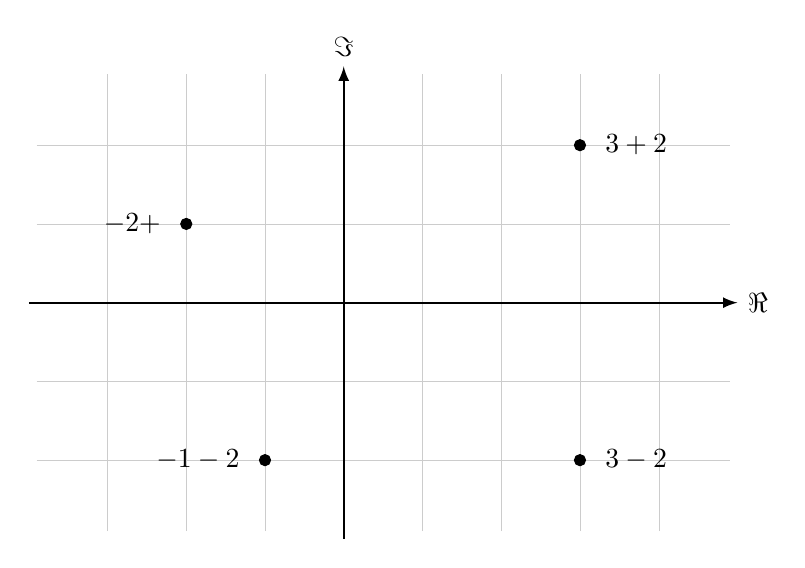
\begin{tikzpicture}[scale=1]
\draw[ultra thin, gray!40] (-3.9,-2.9) grid (4.9,2.9);
\draw[-latex,thick,black] (-4,0) -- (5,0) node[right] {$\Re$};
\draw[-latex,thick,black] (0,-3) -- (0,3) node[above] {$\Im$};
\draw[fill] (3,2) circle (2pt) node[right,xshift=2mm] {$3+\imunit 2$};
\draw[fill] (3,-2) circle (2pt) node[right,xshift=2mm] {$3-\imunit 2$};
\draw[fill] (-2,1) circle (2pt) node[left,xshift=-2mm] {$-2+\imunit$};
\draw[fill] (-1,-2) circle (2pt) node[left,xshift=-2mm] {$-1-\imunit 2$};
\end{tikzpicture}
\caption{Vier punten in het complexe vlak.}
\label{fig:comvierpunten}
\end{figure}


\section{Poolcoördinaten}

Als we nu in het complexe vlak een \textsl{wijzer} tekenen vanuit de oorsprong (het complexe getal $0+\imunit0$) naar het complexe punt $\underline{z}$, dan kunnen we het punt $\underline{z}$ ook uitdrukken in \textsl{poolcoördinaten}. Hierbij worden een lengte vanuit de oorsprong tot aan het punt $\underline{z}$ en een hoek t.o.v.\@ de x-as opgegeven. In figuur~\ref{fig:compuntinhetcomplexevlak} zijn de wijzer en het punt $\underline{z}$ getekend.

\begin{figure}[!ht]
\centering
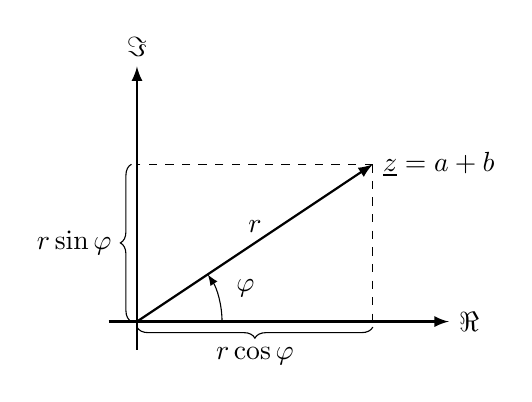
\begin{tikzpicture}[scale=3.6] % scale is radius in cm
\def\uangle{33.7}
\draw[-latex,thick] (0,-0.1) -- (0,0.9) node[above] {$\Im$};
\draw[-latex,thick] (-.1,0) -- (1.1,0) node[right] {$\Re$};
\draw[-latex,thick] (0,0) --(\uangle:1) node[midway,above] {$r$} node[right] {$\underline{z}=a+\imunit b$};
\draw[dashed] (\uangle:1) -| (0,0);
\draw[dashed] (\uangle:1) |- (0,0);
\draw[decorate,decoration={brace,amplitude=4pt,mirror,raise=2pt}] (0,0) -- node[below,yshift=-2mm] {$r\cos\varphi$} ({cos(\uangle)},0);
\draw[decorate,decoration={brace,amplitude=4pt,raise=2pt}] (0,0) -- node[left,xshift=-2mm] {$r\sin\varphi$} (0,{sin(\uangle)});
\draw[-latex] (0.3,0) arc (0:\uangle:0.3);
\node at (\uangle/2:0.4) {$\varphi$};
\end{tikzpicture}
\caption{Een punt in het complexe vlak.}
\label{fig:compuntinhetcomplexevlak}
\end{figure}

De lengte van de wijzer is $r$ en de hoek van de wijzer ten opzichte van de reële as is $\varphi$ (de Griekse letter ``phi''). We kunnen het punt $\underline{z}$ nu ook beschrijven met behulp van de lengte en de hoek:
%
\begin{equation}
\underline{z} = a + \imunit b = r\cos\varphi + \imunit r\sin\varphi = r(\cos\varphi + \imunit\sin\varphi)
\end{equation}
%
We noteren het punt $\underline{z}$ in poolcoördinaten als volgt:
\begin{equation}
r\angle\varphi
\end{equation}
%
Dit wordt de \textsl{Steinmetz-notatie} genoemd. Merk op dat $r\angle\varphi$ een complex getal voorstelt.
We kunnen nu een aantal conversieregels beschrijven. Vanuit poolcoördinaten naar rechthoekcoördinaten:
%
\begin{equation}
\begin{split}
a &= r\cos\varphi \\
b &= r\sin\varphi \\
\end{split}
\end{equation}
Vanuit rechthoekcoördinaten naar poolcoördinaten:
\begin{equation}
\begin{split}
r       &= \sqrt{\mathstrut a^2 + b ^2} \\
\varphi &= \arctan\left(\dfrac{b}{a}\right)
\end{split}
\end{equation}
%
Merk op dat de hoek $\varphi$ doorgaans in radialen wordt gegeven.
Ten aanzien van de poolcoördinaten kunnen we nog het volgende melden:
\begin{itemize}
\item Bij een gelijkblijvende lengte $r$ en een oplopende hoek $\varphi$ beschrijft het punt $\underline{z}$ een \textsl{cirkel} in het complexe vlak.
\item Om de lengte van $\underline{z}$ aan te geven, kunnen absoluutstrepen gebruikt worden: $r=|\underline{z}|$.
\item Bij het punt $\underline{z} = 0 + \imunit0$ is de lengte 0 en de hoek $\varphi$ \textsl{onbepaald}.
\item De hoek $\varphi$ ligt tussen $-\pi$ (niet inclusief) en $\pi$ (inclusief). Voor de hoek $\varphi$ geldt:
\begin{equation}
\varphi = \begin{dcases}
\arctan\left(\frac{b}{a}\right)       & \text{voor } a>0 \\
\arctan\left(\frac{b}{a}\right) + \pi & \text{voor } a<0, b \geq 0 \\
\arctan\left(\frac{b}{a}\right) - \pi & \text{voor } a<0, b < 0 \\
+\dfrac{1}{2}\pi                      & \text{voor } a=0, b > 0 \\
-\dfrac{1}{2}\pi                      & \text{voor } a=0, b < 0 \\
\text{onbepaald}                      & \text{voor } a=0, b = 0
\end{dcases}
\end{equation}
\end{itemize}


